%   % !TEX root = ../../VIII,3_Rahmen-TeX_8-1.tex
%
%
%   Band VIII, 3 N.~??A27
%   Signatur/Tex-Datei: LH_35_14_02_046v,047v
%   RK-Nr. 60653
%   Überschrift: [Zeichnungen zur Bruchfestigkeit]
%   Modul: Mechanik // AEF (Festigkeit)
%   Datierung: [Ende Dezember 1689 bis Frühjahr 1690 (?)]
%   WZ: 803012 = RK-WZ 409 = Kreuz auf drei Kreisen/Ringen in senkr. Reihe, darunter cBv / GBV?
%   SZ: keins
%   Bilddateien (PDF): LH_35_14_02_046v,047v_d1; LH_35_14_02_046v,047v_d2; LH_35_14_02_046v,047v_d3; LH_35_14_02_046v,047v_d4; LH_35_14_02_046v,047v_d5; LH_35_14_02_046v,047v_d6; (insgesamt: ????)
%
%
%
\selectlanguage{ngerman}%
\frenchspacing%
%
 \count\Bfootins=1200
\count\Afootins=1200
\count\Cfootins=1200
\begin{ledgroupsized}[r]{120mm}%
\footnotesize%
\pstart%
\noindent%
\textbf{Überlieferung:}%
\pend%
\end{ledgroupsized}%
\begin{ledgroupsized}[r]{114mm}%
\footnotesize%
\pstart%
\parindent -6mm%
\makebox[6mm][l]{\textit{L}}%
Zeichnungen: LH~XXXV~14,~2 Bl.~46 und LH~XXXV~14,~2 Bl.~47.
Ein unregelmäßig beschnittener und seitlich gerissener Bogen 4\textsuperscript{o}\! (Bl.~46)
und ein davon abgeschnittener Zettel (Bl.~47; 10,7 x 10,1 cm); 
% RK 58241 + RK 58242
ein Wasserzeichen auf Bl.~46 und ein Fragment hiervon auf Bl.~47:
italienisches Papier.
Zwei Seiten: % auf Bl.~46~v\textsuperscript{o} und Bl.~47~v\textsuperscript{o}
auf Bl.~46~v\textsuperscript{o} sind die Diagramme \lbrack\textit{Fig.~1}\rbrack\ und \lbrack\textit{Fig.~4}\rbrack\ bis \lbrack\textit{Fig.~9}\rbrack\ sowie zwei nicht wiedergegebene Entwürfe überliefert;
auf Bl.~47~v\textsuperscript{o} die Diagramme \lbrack\textit{Fig.~2}\rbrack\ und \lbrack\textit{Fig.~3}\rbrack.
Ferner finden sich auf Bl.~46~r\textsuperscript{o}\! Auszüge aus Galileis \textit{Discorsi} (die noch in \textit{LSB} VIII zu edieren sind)
und auf Bl.~47 das Stück N.~29.%
\protect\index{Namensregister}{\textso{Galilei} (Galilaeus, Galileus), Galileo 1564\textendash1642}
\pend%
\end{ledgroupsized}%
%
\vspace{5mm}%
\begin{ledgroup}%
\footnotesize%
\pstart%
\noindent%
\textbf{Datierungsgründe:}
Die Verwendung des Papiers, auf dem das vorliegende Stück N.~30 % nebst der Aufzeichnung N.~??A26 und Auszügen aus Galileis \textit{Discorsi} 
überliefert ist, ist im Leibniz-Nachlass nach heutigem Wissensstand lediglich für den Zeitraum zwischen Ende Dezember 1689 und spätestens Januar 1691 belegt (siehe die Datierungsgründe von N.~29, S.~\pageref{LH_35_14_02_047_datierung}).
Die zu N.~30 gehörigen Zeichnungen \lbrack\textit{Fig.~2}\rbrack\ und \lbrack\textit{Fig.~3}\rbrack\
% sind auf demselben Träger wie der Text N.~??A26 überliefert und 
wurden aber bei der Abfassung der mit überlieferten Aufzeichnung N.~29 überschrieben.
% N.~??A26 ist nach Ende Dezember 1689 verfasst worden.
Folglich muss N.~30 zwischen Ende Dezember 1689 und der Abfassung von N.~29 entstanden sein.
Daraus ergibt sich die vorgeschlagene Datierung.
\pend%
\end{ledgroup}%
%
\selectlanguage{latin}%
\frenchspacing%
%
%
\vspace{8mm}
\pstart%
\noindent
\normalsize
[46v\textsuperscript{o}]
\pend
%
%
  \vspace*{0.0em}
  \centerline{\includegraphics[width=0.36\textwidth]{gesamttex/edit_VIII,3/images/LH_35_14_02_046v,047v_d1.pdf}}%
  \vspace*{0.5em}
  \centerline{\lbrack\textit{Fig.~1}\rbrack}%
  \label{LH_35_14_02_046v,047v_Fig.1}%
  \vspace{1.5em}%
%
%
\pstart%
\noindent
\normalsize
[47~v\textsuperscript{o}]
\pend
 \vspace{0.2em}
\pstart 
\begin{minipage}[t]{0.5\textwidth}
\includegraphics[width=0.58\textwidth]{gesamttex/edit_VIII,3/images/LH_35_14_02_046v,047v_d2.pdf}
\end{minipage}
\hspace{10mm}
\begin{minipage}[t]{0.5\textwidth}
\includegraphics[width=0.58\textwidth]{gesamttex/edit_VIII,3/images/LH_35_14_02_046v,047v_d3.pdf}
\end{minipage}\vspace{-0.5em}
\\
\hspace*{21mm} [\textit{Fig.~2}] \label{LH_35_14_02_046v,047v_Fig.2}\hspace*{67mm} [\textit{Fig.~3}] \label{LH_35_14_02_046v,047v_Fig.3}
\pend
%%
%%
% 
%  \centerline{\hspace*{-60mm}\includegraphics[width=0.28\textwidth]{gesamttex/edit_VIII,3/images/LH_35_14_02_046v,047v_d2.pdf}}%
%  \vspace*{-0.5em}
%  \centerline{\hspace*{-60mm}\lbrack\textit{Fig.~2}\rbrack}%
%  \label{LH_35_14_02_046v,047v_Fig.2}%
%%  \vspace*{1.5em}%
%%
%  \vspace*{-6.5em}
%  \centerline{\hspace*{60mm}\includegraphics[width=0.28\textwidth]{gesamttex/edit_VIII,3/images/LH_35_14_02_046v,047v_d3.pdf}}%
%  \vspace*{-0.5em}
%  \centerline{\hspace*{60mm}\lbrack\textit{Fig.~3}\rbrack}%
%  \label{LH_35_14_02_046v,047v_Fig.3}%
%%  \vspace*{1.5em}%
  \newpage%
%
%
\pstart%
\noindent
\normalsize
[46v\textsuperscript{o}]
\pend
\pstart\hspace{5mm}
\begin{minipage}[b][30mm][t]{0.5\textwidth}
\includegraphics[width=0.6\textwidth]{gesamttex/edit_VIII,3/images/LH_35_14_02_046v,047v_d4.pdf}
\end{minipage}
\hspace{5mm}
\begin{minipage}[b][30mm][b]{0.5\textwidth}
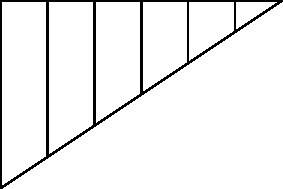
\includegraphics[width=0.5\textwidth]{gesamttex/edit_VIII,3/images/LH_35_14_02_046v,047v_d5.pdf}
\end{minipage}
\pend
\vspace{11mm}
\pstart
\hspace*{21mm} [\textit{Fig.~4}] \label{LH_35_14_02_046v,047v_Fig.4}\hspace*{56mm} [\textit{Fig.~5}] \label{LH_35_14_02_046v,047v_Fig.5}
\pend
\vspace{3em}
%
%%
%%
%  \vspace*{0.0em}
%  \centerline{\hspace*{-55mm}\includegraphics[width=0.26\textwidth]{gesamttex/edit_VIII,3/images/LH_35_14_02_046v,047v_d4.pdf}}%
%  \vspace*{0.0em}
%  \centerline{\hspace*{-55mm}\lbrack\textit{Fig.~4}\rbrack}%
%  \label{LH_35_14_02_046v,047v_Fig.4}%
%%  \vspace*{2.0em}%
%%
%  \vspace*{-11.0em}
%  \centerline{\hspace*{65mm}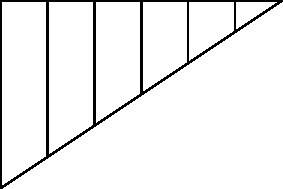
\includegraphics[width=0.24\textwidth]{gesamttex/edit_VIII,3/images/LH_35_14_02_046v,047v_d5.pdf}}%
%  \vspace*{0.0em}
%  \centerline{\hspace*{65mm}\lbrack\textit{Fig.~5}\rbrack}%
%  \label{LH_35_14_02_046v,047v_Fig.5}%
%%  \vspace*{2.0em}%
%
\pstart\setline{1}\hspace{6mm}
\begin{minipage}[t]{0.33\textwidth}\vspace{-17mm}
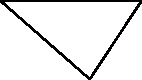
\includegraphics[width=0.38\textwidth]{gesamttex/edit_VIII,3/images/LH_35_14_02_046v,047v_d6.pdf}
\end{minipage}
\hspace{2mm}
\begin{minipage}[t]{0.33\textwidth}
\includegraphics[width=0.22\textwidth]{gesamttex/edit_VIII,3/images/LH_35_14_02_046v,047v_d7.pdf}
\end{minipage}
\hspace{-9mm}
\begin{minipage}[t]{0.33\textwidth}
\includegraphics[width=0.65\textwidth]{gesamttex/edit_VIII,3/images/LH_35_14_02_046v,047v_d8.pdf}
\end{minipage}\vspace{-0.5em}
\\
\\
\hspace*{17mm} [\textit{Fig.~6}]\label{LH_35_14_02_046v,047v_Fig.6}\hspace*{31mm} [\textit{Fig.~7}]\label{LH_35_14_02_046v,047v_Fig.7}\hspace*{34mm} [\textit{Fig.~8}]\label{LH_35_14_02_046v,047v_Fig.8}
\vspace{1.5em}
\pend
%  \vspace*{10.0em}
%  \centerline{\hspace*{-85mm}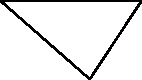
\includegraphics[width=0.11\textwidth]{gesamttex/edit_VIII,3/images/LH_35_14_02_046v,047v_d6.pdf}}%
%  \vspace*{0.5em}
%  \centerline{\hspace*{-85mm}\lbrack\textit{Fig.~6}\rbrack}%
%  \label{LH_35_14_02_046v,047v_Fig.6}%
%%  \vspace*{15em}%
%%
%  \vspace*{-8.0em}
%  \centerline{\includegraphics[width=0.075\textwidth]{gesamttex/edit_VIII,3/images/LH_35_14_02_046v,047v_d7.pdf}}%\hspace*{-5mm}
%  \vspace*{0.5em}
%  \centerline{\lbrack\textit{Fig.~7}\rbrack}%\hspace*{-5mm}
%  \label{LH_35_14_02_046v,047v_Fig.7}%
%%  \vspace*{15em}%
%%
%  \vspace*{-10.0em}
%  \centerline{\hspace*{85mm}\includegraphics[width=0.23\textwidth]{gesamttex/edit_VIII,3/images/LH_35_14_02_046v,047v_d8.pdf}}%\hspace*{-5mm}
%  \vspace*{0.0em}
%  \centerline{\hspace*{85mm}\lbrack\textit{Fig.~8}\rbrack}%
%  \label{LH_35_14_02_046v,047v_Fig.8}%
%%  \vspace*{15em}%
%
\vspace{4.5em}
   \centerline{\includegraphics[width=0.41\textwidth]{gesamttex/edit_VIII,3/images/LH_35_14_02_046v,047v_d9.pdf}}%\hspace*{-5mm}
  \vspace{0.5em}
  \centerline{\lbrack\textit{Fig.~9}\rbrack}%
  \label{LH_35_14_02_046v,047v_Fig.9}%
%  \vspace*{15em}%
%
%
%%%%    ENDE DES STÜCKS AUF S. 46V